\section{Introduction}

The scientific community is currently experiencing a surge in interest in techniques offering higher spatial resolution, a trend intrinsically linked with advancements in technology. Since the pioneering contributions of \citet{Egli2000}, the implementation of high-resolution scanning magnetic microscopy (SMM) methodologies has become increasingly feasible in paleomagnetic research, offering an alternative to conventional approaches that typically analyze entire rock samples. This method facilitates the discernment of magnetization heterogeneities undetectable at larger scales. Nonetheless, these SMM techniques require data processing to unravel the information contained in the potential field measured. Dealing with potential fields, in general, could be very challenging due to the ambiguity associated with the data itself generating non-unique results during the inversion \citep{Blakely1996}. A common way to circumvent the non-uniqueness is integrating prior knowledge about the sources causing the anomaly such as the position of a known magnetized source \citep{Fabian2019}. The X-ray computed tomography (microCT) technique is a good example of the application of the additional information \citep[\textit{e.g.}][]{DeGroot2018, DeGroot2021, Koster2023}, which can be further refined by the inversion of the magnetic moment using spherical harmonic \citep[\textit{e.g.}][]{CortesOrtuno2021, CortesOrtuno2022}.

Another way to insert additional information without the requirement of performing new measurements was proposed by \citet{Souza-Junior2023b}, which uses techniques extrapolated from aeromagnetic surveys, such as the Euler deconvolution, due to its similarity with the SMM \citep{Weiss2007}. The methodology is designed for the semi-automatic estimation of position and dipole moments for individual grains and consists of three main steps. First, it combines classic potential field data processing (like total gradient amplitude) with image processing techniques (such as histogram stretching, and edge detection) to identify and isolate the magnetic fields of individual sources into data windows. Next, the 3D position of the source is estimated through the Euler deconvolution equation based on the magnetic microscopy field measurements within each data window. Finally, the 3-component dipole moment vector is obtained using a least-square estimator assuming that a dipolar source causes the magnetic anomaly. The methodology was originally designed for computational efficiency and stability. However, it infringes on the mathematical premise of inversion theory states that the sampled area must be encapsulated by inversion domain \citep{Baratchart2013, Lima2013} thus, more often than not, failing to account for the mutual interference between sources and/or shifts in the measured field. This study introduces a novel approach that aims to account for the mutual interference of the sources in the methodology proposed by \citet{Souza-Junior2023b}, as well as any shift in the field. Through refining the window-based approach, the proposed methodology presents a significant advancement in magnetic microscopy, with potential application for paleomagnetic studies. 

% the window-based approach, which despite its promising initial implications, proved susceptible to undesired influences, compromising the accuracy of position and dipole moment estimations in determined situations. These unexpected findings shed critical light on the methodology used and ultimately caused the motivation to explore new horizons and the development of a substantially more robust and accurate approach.






% it recognizes the challenge of potential interference from stronger magnetic sources on the estimated positions of weaker nearby sources, underscoring the importance of accounting for source interactions to accurately determine their magnetic parameters and positions.

% aims to achieve the semi-automatic estimation of dipole moments for individual grains, this is approached through a three-part methodology:

% \begin{enumerate}
%     \item \textbf{Data preprocessing:} Apply classic potential field data processing techniques, including the total gradient amplitude map (TGA). Employ image processing methods, such as histogram stretching, and an edge detection algorithm to identify and spatially isolate the magnetic field of each source into window data.

%     \item \textbf{3D position estimation:} Estimate the 3D position of magnetic particles by applying the Euler deconvolution method to the data segment identified in the first step.

%     \item \textbf{Magnetic moment inversion:} Execute the magnetic moment inversion in the data segment to determine the 3-component dipole moment vector. Which assumes a dipole model located in the position estimated with the Euler equation. 
% \end{enumerate}

% Performing the inversion separately for each data segment enhances computational efficiency, ensuring a quick solution to the linear inverse problem. However, it is important to acknowledge that stronger magnetic sources may influence the estimated positions and magnetic moment of nearby weaker ones. This understanding is crucial for refining the estimation process and ensuring robust results in magnetic parameter estimation.

%%%%%%%%%%%%%%%%%%%%%%%%%%%%%%%%%%%%%%%%%%%%%%%%%%%%%%%%%%%%%%%%%%%%%%%%%%%%%%%
\section{Methodology}

% The methodology proposed by \citet{Souza-Junior2023b} aimed to achieve the semi-automatic estimation of dipole moments for individual grains per image. This is approached through a three-part methodology. The initial step involves the application of classic potential field data processing, such as total gradient amplitude, coupled with image processing techniques like histogram stretching, equalization, and an edge detection algorithm. This enables the identification and spatial isolation of the magnetic field caused by each source. 

% Following that, attention shifts to the estimation of the 3D position of magnetic particles based on magnetic field measurements. This is carried out by applying the Euler deconvolution method to the data segment identified in the first step. In the final phase, the magnetic moment inversion process is executed. This entails estimating the 3-component dipole moment vector by inverting the magnetic field data assuming a dipolar model. The inversion is conducted separately for each data segment identified initially, which in theory ensures stability and computational efficiency in solving the linear inverse problem in a few seconds. 

% However, estimating the source's position based on Euler deconvolution revealed that stronger magnetic sources may influence the estimated positions of nearby weaker ones. Therefore, it becomes imperative to consider the interplay among the sources to estimate their magnetic parameters and position accurately. Understanding how these magnetic sources interact with each other is crucial for refining our estimation process and ensuring robust results in magnetic parameter estimation.


To fully leverage the advancement of magnetic microscopy for paleomagnetic studies, we must isolate the individual contribution of the stable remnant magnetization carriers within the rock fabric. This is also related to a major limitation of the inversion procedures used to retrieve the information carried by these grains. To guarantee the solution's uniqueness, prior information about the sources must be provided. The novelty of Euler deconvolution application to magnetic microscopy data, developed by \citet{Souza-Junior2023b}, showed the possibility of individual estimation of magnetic grains without additional measurements. However, the technique violates the principles of inverse theory by ignoring non-encapsulated effects within the inversion domain, \textit{i.e.} mutual influence of sources. This study explores a new methodology to effectively manage interfering sources during the inversion process, which is designed to mitigate the magnetic sources' interference and enhance the precision of the inversion analyses proposed.

\subsection{Sources detection}
The first step in enhancing the technique involves source detection. To account for mutual interference between magnetic carriers, the algorithm must reliably identify the data window associated with each grain. There are many techniques ...
 
 Yago's problem

\subsection{Magnetic vector inversion with interfering sources}\label{inversion-section}

The interference source methodology is proposed to enhance the accuracy of window-based inversion analyses in magnetic data, particularly in scenarios where stronger magnetic fields could introduce distortions in the results. \textcolor{red}{As mentioned earlier, the edge detection algorithm is applied to the total gradient anomaly map to segment the data windows of the magnetic sources, which follow the descending order of blob magnitude (Yago)}. The latter is directly proportional to the magnetic signal of the sources, hence it might be used to account for the effect of stronger sources. This process is divided into distinct steps:


\subsubsection{Position estimation}
    Euler deconvolution (ED) is widely applied in aeromagnetic surveys \citep{Barbosa2011, Melo2013, Melo2018} to obtain a 3D position estimation \cite[after][]{Reid1990}. The only assumption is the source's shape given by the structural index ($\eta$), in the case of a dipole $\eta = 3$. The Euler's homogeneity equation is then given by
    
        \begin{equation}
        \label{eq_euler_homogeneity}
        (x - x_c)\partial_x f
        + (y - y_c)\partial_y f
        + (z - z_c)\partial_z f
        = (b - f)\eta
        \ .
        \end{equation}
    
    \noindent{The solution of the ED is performed in the rearranged pseudo-parametric model}
    
    \begin{equation}
    x_c \partial_x f + y_c \partial_y f + z_c \partial_z f + \eta b
    =
    x \partial_x f + y \partial_y f + z \partial_z f + \eta f
    \ .
    \end{equation}
    
    For a given magnetic field anomaly ($f$) and its directional derivatives ($\partial \alpha f$, $\alpha = x, y, z$ ) at the i\textsuperscript{th} observation point ($x_i, y_i, z_i$), $i=1, 2,..., N$, we can describe an $N \times 4$ system of equations as:
    
    \begin{equation}
    {\overbrace{
    \begin{bmatrix}
      {\partial_x f}_1 & {\partial_y f}_1 & {\partial_z f}_1 & \eta \\
      {\partial_x f}_2 & {\partial_y f}_2 & {\partial_z f}_2 & \eta \\
      \vdots & \vdots & \vdots & \vdots \\
      {\partial_x f}_N & {\partial_y f}_N & {\partial_z f}_N & \eta
    \end{bmatrix}
    }^{\mathbf{G}}}_{N \times 4}
    {\overbrace{
    \begin{bmatrix}
      x_c \\ y_c \\ z_c \\ b
    \end{bmatrix}
    }^{\mathbf{p}}}_{4 \times 1}
    =
    {\overbrace{
    \begin{bmatrix}
      x_1 {\partial_x f}_1 + y_1 {\partial_y f}_1 + z_1 {\partial_z f}_1 + \eta f_1 \\
      x_2 {\partial_x f}_2 + y_2 {\partial_y f}_2 + z_2 {\partial_z f}_2 + \eta f_2 \\
      \vdots \\
      x_N {\partial_x f}_N + y_N {\partial_y f}_N + z_N {\partial_z f}_N + \eta f_N \\
    \end{bmatrix}
    }^{\mathbf{h}}}_{N \times 1}
    \ .
    \end{equation}
    
    The solution of this linear system is defined by the vector $\mathbf{p}$ that minimizes the misfit function $\phi(\mathbf{p})$, given by the sum of the squared differences between the pseudo-observation data ($\mathbf{h}^o$) and the predicted data ($\mathbf{h}$):
    
    \begin{equation}
    \label{function_phi}
    \phi(\mathbf{p}) = \min_{\mathbf{p}} \| \mathbf{G}\mathbf{p} - \mathbf{\mathbf{h}^o} \|_2^2\ = \min_{\mathbf{p}} \| \mathbf{h} - \mathbf{\mathbf{h}^o} \|_2^2\
    .
    \end{equation}
    
    \noindent{Which is obtained by applying}
    
    \begin{equation}
    \label{euler_solution}
    \mathbf{p} = {[\mathbf{G}^T \mathbf{G}]}^{-1} [\mathbf{G}^T \mathbf{h}^o]\ .
    \end{equation}
    
    The parameters vector $\mathbf{p}$ contains the dipolar source's coordinates, $x_c$, $y_c$, and $z_c$. It also contains the base level ($b$), the background field within the window.
    
\subsubsection{Magnetic moment inversion} 
    One of the main drawbacks of estimating a physical property from potential data, such as the dipole moment vector $(m_x, m_y, m_z)$, lies in its ambiguity \citep{Blakely1996}. This is commonly circumvented by adding additional information about the sources (\textit{e.g.} shape, position, and size). Therefore, the ED solution (Equation~\ref{euler_solution}) might be used as prior information to recover the dipole moment of the sources causing the anomaly within the window data.
    
     Following \citet{Oliveira2015Estimation}, the vertical component of the magnetic field ($fz$), measured at the i\textsuperscript{th} observation point ($i=1, 2, ..., N$), produced by a dipolar source located in the Cartesian coordinates $x_c, y_c$ and $z_c$, can be calculated using:

     \begin{equation}
    \label{eq_dipole_bz}
    {\overbrace{\begin{bmatrix}
    \dfrac{\mu_0}{4\pi} \dfrac{\partial^2}{\partial z \partial x} \dfrac{1}{r_i}
    & \dfrac{\mu_0}{4\pi} \dfrac{\partial^2}{\partial z \partial y} \dfrac{1}{r_i}
    & \dfrac{\mu_0}{4\pi} \dfrac{\partial^2}{\partial z \partial z} \dfrac{1}{r_i}
    \end{bmatrix}}^{\mathbf{A}}}_{N \times 3}
    {\overbrace{{\begin{bmatrix}
    m_x \\ m_y \\ m_z
    \end{bmatrix}}}^{\mathbf{m}}}_{3 \times 1}
    =
    ~{\overbrace{\begin{bmatrix}
    fz_i
    \end{bmatrix}}^{\mathbf{d}}}_{N \times 1}
    \ .
    \end{equation}

    \noindent{
    Where $r = \sqrt{(x_i - x_c)^2 + (y_i - y_c)^2 + (z_i - z_c)^2}$ is the distance between the observation point $(x_i, y_i, z_i)$ and the dipolar source $(x_c, y_c, z_c)$, $\mu_0$ is the vacuum magnetic permeability, and the second-order derivatives terms in Equation~\ref{eq_dipole_bz} are:
    
    \begin{equation}
    \begin{aligned}
    \dfrac{\partial^2}{\partial z \partial x} \dfrac{1}{r_i} &=
    \dfrac{3(z_i - z_c)(x_i - x_c)}{{r_i}^5}\ ,
    \\
    \dfrac{\partial^2}{\partial z \partial y} \dfrac{1}{r_i} &=
    \dfrac{3(z_i - z_c)(y_i - y_c)}{{r_i}^5}\ ,
    \\
    \dfrac{\partial^2}{\partial z \partial z} \dfrac{1}{r_i} &=
    \dfrac{3(z_i - z_c)^2}{{r_i}^5} - \dfrac{1}{{r_i}^3}\ .
    \end{aligned}
    \end{equation}}

    The $N \times 3$ linear system in the Equation~\ref{eq_dipole_bz} has its solution defined by the parameter vector ($\mathbf{m}$) that minimizes the misfit function $\psi(\mathbf{m})$ given by the residual between the predicted ($\mathbf{\mathbf{d}}$) and observed ($\mathbf{\mathbf{d}^o}$) data vectors. The latter is also corrected by the background field ($b$) obtained with the ED. Then the misfit function $\psi(\mathbf{m})$ can be written as:
   
    \begin{equation}
    \label{psi_function}
    \psi(\mathbf{m}) = \min_{\mathbf{m}} \| \mathbf{A}\mathbf{m} - \mathbf{\mathbf{d}^o} \|_2^2\ = \min_{\mathbf{m}} \| \mathbf{d} - (\mathbf{\mathbf{d}^o}-b) \|_2^2\
    .
    \end{equation}

    The parameters vector ($\mathbf{m}$), containing the Cartesian components of the magnetic moment, can be obtained by the least-squares estimator:

    \begin{equation}
    \label{dipole_moment_solution}
    \mathbf{m} = {[\mathbf{A}^T \mathbf{A}]}^{-1} [\mathbf{A}^T (\mathbf{d}^o - b)]\ .
    \end{equation}
        
\subsubsection{Simplex optimization} 
     The forward model of the dipole's vertical component anomaly from the Equation~\ref{eq_dipole_bz} can be rewritten as:

    \begin{equation}
        \small
        \label{bz_dipole_equation}
        {d}_{i} = \frac{\mu_0}{4 \pi} \left [ 3 \frac{ (z_i-z_c) \left ( m_x (x_i-x_c) + m_y (y_i-y_c) + m_z (z_i-z_c) \right )}{{r_i}^5} - \frac{m_z}{{r_i}^3} \right ] .
    \end{equation}
    
     After obtaining the initial estimates of the 3D position $(x_{c0}, y_{c0}, z_{c0})$ and the dipole moment vector $(m_{x0}, m_{y0}, m_{z0})$, both position and magnetic moment might still be refined to improve the model results. For this process, the optimization technique utilized was the Scipy Nelder-Mead method \citep{2020SciPy-NMeth}, which employs these six parameters obtained in previous steps as initial guesses for the goal function (Equation~\ref{bz_dipole_equation}). The misfit function to be minimized is given by:
    
    \begin{equation}
    \label{misfit_equation}
    \xi (x_c, y_z, z_c, m_x, m_y, m_z) = \| (\mathbf{d}^{o}-b) - \mathbf{d} \|^2.
    \end{equation} 
    
     The Nelder-Mead method, a gradient-free optimization technique, systematically searches the optimal solution of Equation~\ref{misfit_equation} by iteratively adjusting a simplex in the parameter space \citep{Nelder-Mead1965}. This is particularly useful for optimizing functions where gradients are difficult to compute or unavailable. 
     
     However, the substantial difference of up to seven orders of magnitude between the position and the magnetic moment poses a challenge. This dissimilarity directly affects the simplex operations and has been addressed by normalizing the initial magnetic moment magnitude ($m_0 = \sqrt{{m_{x0}}^2+{m_{y0}}^2+{m_{z0}}^2}$), as follows:
     \begin{align}
    \label{normalizing_m_parameters}
    {m_x}^{j+1} &= \frac{{m_x}^{j}}{m_0}, & {m_y}^{j+1} &= \frac{{m_y}^{j}}{m_0}, & \text{and} & &{m_z}^{j+1} &= \frac{{m_z}^{j}}{m_0}
    \ .
    \end{align}
     
\noindent{Which was also applied for the position vector using the initial position estimates:}
     \begin{align}
    \label{normalizing_h_parameters}
    {x_c}^{j+1} &= \frac{{x_c}^{j}}{x_{c0}}, & {y_c}^{j+1} &= \frac{{y_c}^{j}}{y_{c0}}, & \text{and} & &{z_c}^{j+1} &= \frac{{z_c}^{j}}{z_{c0}}
    \ .
    \end{align}
    
% \begin{align}
% \label{normalizing_parameters}
% {x_c}^{j+1} &= \frac{{x_c}^{j}}{x_{c0}}, & {y_c}^{j+1} &= \frac{{y_c}^{j}}{y_{c0}}, & \text{and} & &{z_c}^{j+1} &= \frac{{z_c}^{j}}{z_{c0}} \\
% {m_x}^{j+1} &= \frac{{m_x}^{j}}{m_0}, & {m_y}^{j+1} &= \frac{{m_y}^{j}}{m_0}, & \text{and} & &{m_z}^{j+1} &= \frac{{m_z}^{j}}{m_0}
% \ .
% \end{align}

\noindent{These normalization procedures ensure that each parameter falls within a unit range for a given number M of iterations of the simplex optimization, $j = 1,2,..., M$.}
     

\subsubsection{Signal removal} 
    The logical route to account for mutual interference between magnetic sources would be solving the magnetic moment for the whole of the sources at the same time. However, this approach raises three problems:
    \begin{enumerate}
        \item \textbf{The size of the problem:} We would have a linear problem $N \times 3L$ ($L$ is the number of sources) in Equation~\ref{eq_dipole_bz}. This would not pose a problem if the magnetic microscopy data did not include a large number of observation points, potentially encompassing hundreds to thousands of identified sources. Therefore, working with sliced windowed data is much faster.
        
        \item \textbf{Background field correction:} In the proposed methodology, correction for the background field ($b$) eliminates the need for preprocessing the data for regional-residual separation to remove the effects of shifts in the magnetic data. This application is feasible because $b$ is also provided by the ED solution when using windowed data.
        
        \item \textbf{No visible advantage over windowed data}: Tests with synthetic data \textcolor{red}{(see supplementary files)} showed no significant advantage over windowed data. The latter performed significantly better in the benchmark.

    \end{enumerate}
    
    Considering the above, to keep using the window-based approach we propose a sequential subtraction of the influence of the magnetic carriers. For such, the analytical magnetic signal associated with the identified source was computed using a dipole forward model (Equation~\ref{bz_dipole_equation}), with the aid of Choclo python library \citep{choclo2022}, and the simplex optimized parameter vector. This yielded a theoretical representation of the expected magnetic effects for each identified source. This strong source's analytical signal was selectively removed from the dataset. This leads to a dataset devoid of the (the current step) stronger source influence, allowing for gradual isolation of the contributions of weaker sources. This updated dataset also recalculated the directional derivatives for the next Euler deconvolution position estimation.

    This step-by-step procedure is subsequently employed for all detected particles in the sample, from the strongest to the weakest. This led to an improved position estimation compared to the original methodology. This novelty methodology, designed to mitigate the impact of stronger sources and with a better estimation of positions, significantly enhances the precision of subsequent inversion analyses. However, a trade-off between achieving better results and incurring longer computational runtime is unavoidable.

\subsection{Residual anomaly detection}
   The magnetization signal of materials is directly dependent on their volumes. In a rock fabric, this can result in a wide range of particle diameter distributions, from small, stable recording grains (single domain, SD, around 60 nm) to less reliable magnetic carriers (multi-domain, MD, greater than 1000 nm). This results in a significant contrast in the magnetic signal measured using the magnetic microscope. This effect is evident in the synthetic example shown in Figure~\ref{method-redetection}a, which features dipolar sources with a magnetic moment contrast spanning 5 orders of magnitude. 
   
    In the original methodology, sources are initially identified for window selection using a total gradient anomaly (TGA) map, with contrast stretched to highlight sources of varying intensities (both strong and weak) as shown in Figure~\ref{method-redetection}b. However, due to the high signal contrast, this approach proved insufficient for identifying all relevant sources. To address this issue, the procedure outlined in Section~\ref{inversion-section} was implemented to obtain a residual anomaly map. Reapplying the source detection algorithm to this new map enabled the identification of weaker sources (Figure~\ref{method-redetection}c), as the signal from stronger sources was effectively removed. This improvement resulted from the reduced disparity between the signals of weaker magnetic sources and the residual anomalies from each window inversion.

    \begin{figure}[tb!]
      \centering
      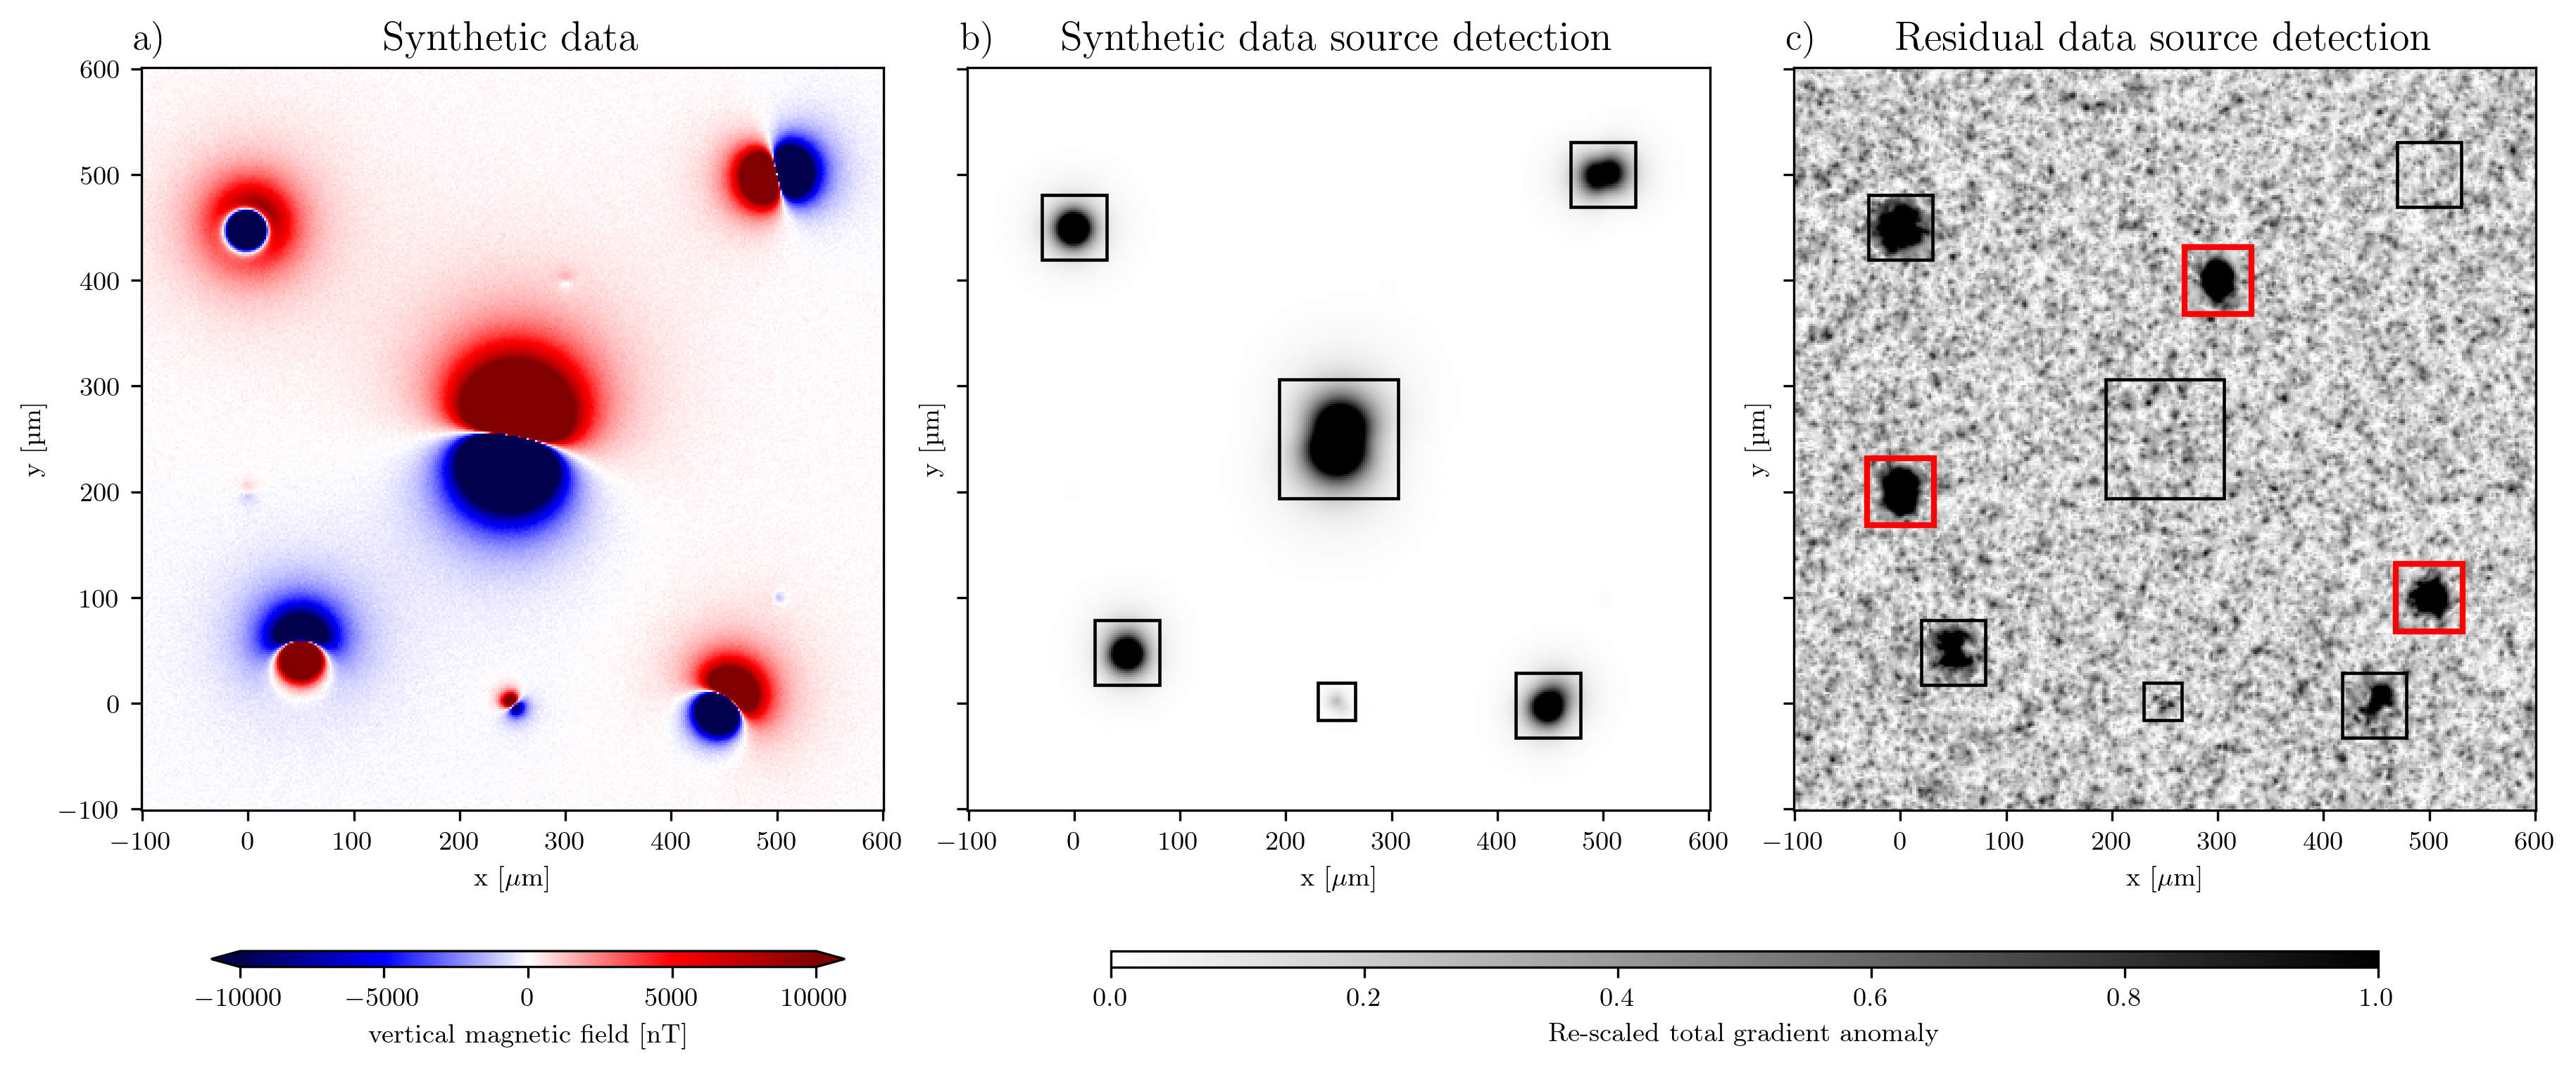
\includegraphics[width=1\linewidth]{paper/figures/re-detection-methodology.png}
      \caption{Workflow to perform the source detection on the residual anomaly. a) Synthetic sample featuring a wide range of magnetic moment intensity. b) The Blob detection algorithm result uses the total gradient obtained with the vertical component of the magnetic field. c) Blob detection algorithm result using the total gradient of the residual anomaly.}
      \label{method-redetection}
    \end{figure}

\section{Synthetic data application}
% As mentioned, this study aims to deal with the mutual interference between the magnetic sources. 
The proposed methodology was applied to complex synthetic data to assess the algorithm's performance. The inversion workflow was tested for its efficiency in the presence of interfering sources for further comparison with the methodology proposed by \citet{Souza-Junior2023b}.

\subsection{Method validation with interfering sources}

The model scenario features several dipole sources with different moment magnitudes, inclinations, and declinations, clustered into two groups. The first group contains dipoles with random orientations, while the second group has a stable direction and moment magnitudes two orders of magnitude smaller than those in the first group. The vertical magnetic field ($b_z$) generated by these sources is corrupted by high-frequency noise to simulate real-world magnetic microscopy data. Additionally, a positive shift is applied to the magnetic field data to mimic the acquisition process in magnetic microscopy with a shifted baseline. This scenario provides insights into the algorithm's robustness and accuracy when faced with a systematically shifted magnetic field, as encountered in certain microscopic magnetic data acquisition setups. 

To evaluate the method, we simulate a complex scenario with 200 magnetic sources randomly distributed across a synthetic thin section measuring $\qty{2000}{\um} \times \qty{2000}{\um}$. The synthetic $b_z$ data are generated on a regular grid with $\qty{2}{\um}$ spacing and a sensor-sample distance of $\qty{5}{\um}$. To enhance realism, we incorporate high-frequency pseudo-random noise with a zero mean and a standard deviation of $\qty{50}{\nano\tesla}$. The first group of sources ($N = 150$) is sampled from a distribution with randomized directions, while the second group ($N = 30$) is sampled from a distribution with a mean declination of $D = \ang{340}\pm\ang{5}$ and an inclination of $I = \ang{35}\pm\ang{5}$. All modeled sources have depths ranging from 1 to $\qty{20}{\um}$. Furthermore, to emulate the complexities observed in real data measurements, a manual background shift of $\qty{2000}{\nano\tesla}$ is introduced.

In real ferromagnetic particles, the Natural Remanent Magnetization (NRM) exhibits individual variations but tends to align with the inducing field direction. The dipole moment directions from two pseudo-random Gaussian distributions were sampled to capture this variability in our synthetic data.

This synthetic data inversion was solved using the standard method \citep{Souza-Junior2023b} and the proposed interfering sources methodology. A summary of the comparison between the classic Euler method and the iterative approach revealed noteworthy results in the context of the analysis of the provided synthetic data. Upon applying the iterative Euler deconvolution method, a significant enhancement in the precision of the magnetic source position is observed when compared to the Euler deconvolution in the standard method. Figure~\ref{euler2}a illustrates the 99 detected sources from the 103 originally modeled, showcasing the algorithm's effectiveness in identifying regions of interest. Figures ~\ref{euler2}b and ~\ref{euler2}c show the results obtained by the standard and iterative Euler methods, respectively. Although, in both cases, the Euler deconvolution is unaffected by the presence of a shift in the magnetic field, it becomes evident that the iterative method yields more accurate and refined estimates. This increase in accuracy is crucial, especially in scenarios where stronger magnetic sources can distort the magnetic field anomaly of weaker sources. Although this new methodology can markedly increase the accuracy in the estimated position for virtually all sources, the biggest errors are still related to clustered sources.


\begin{figure}[tb!]
  \centering
  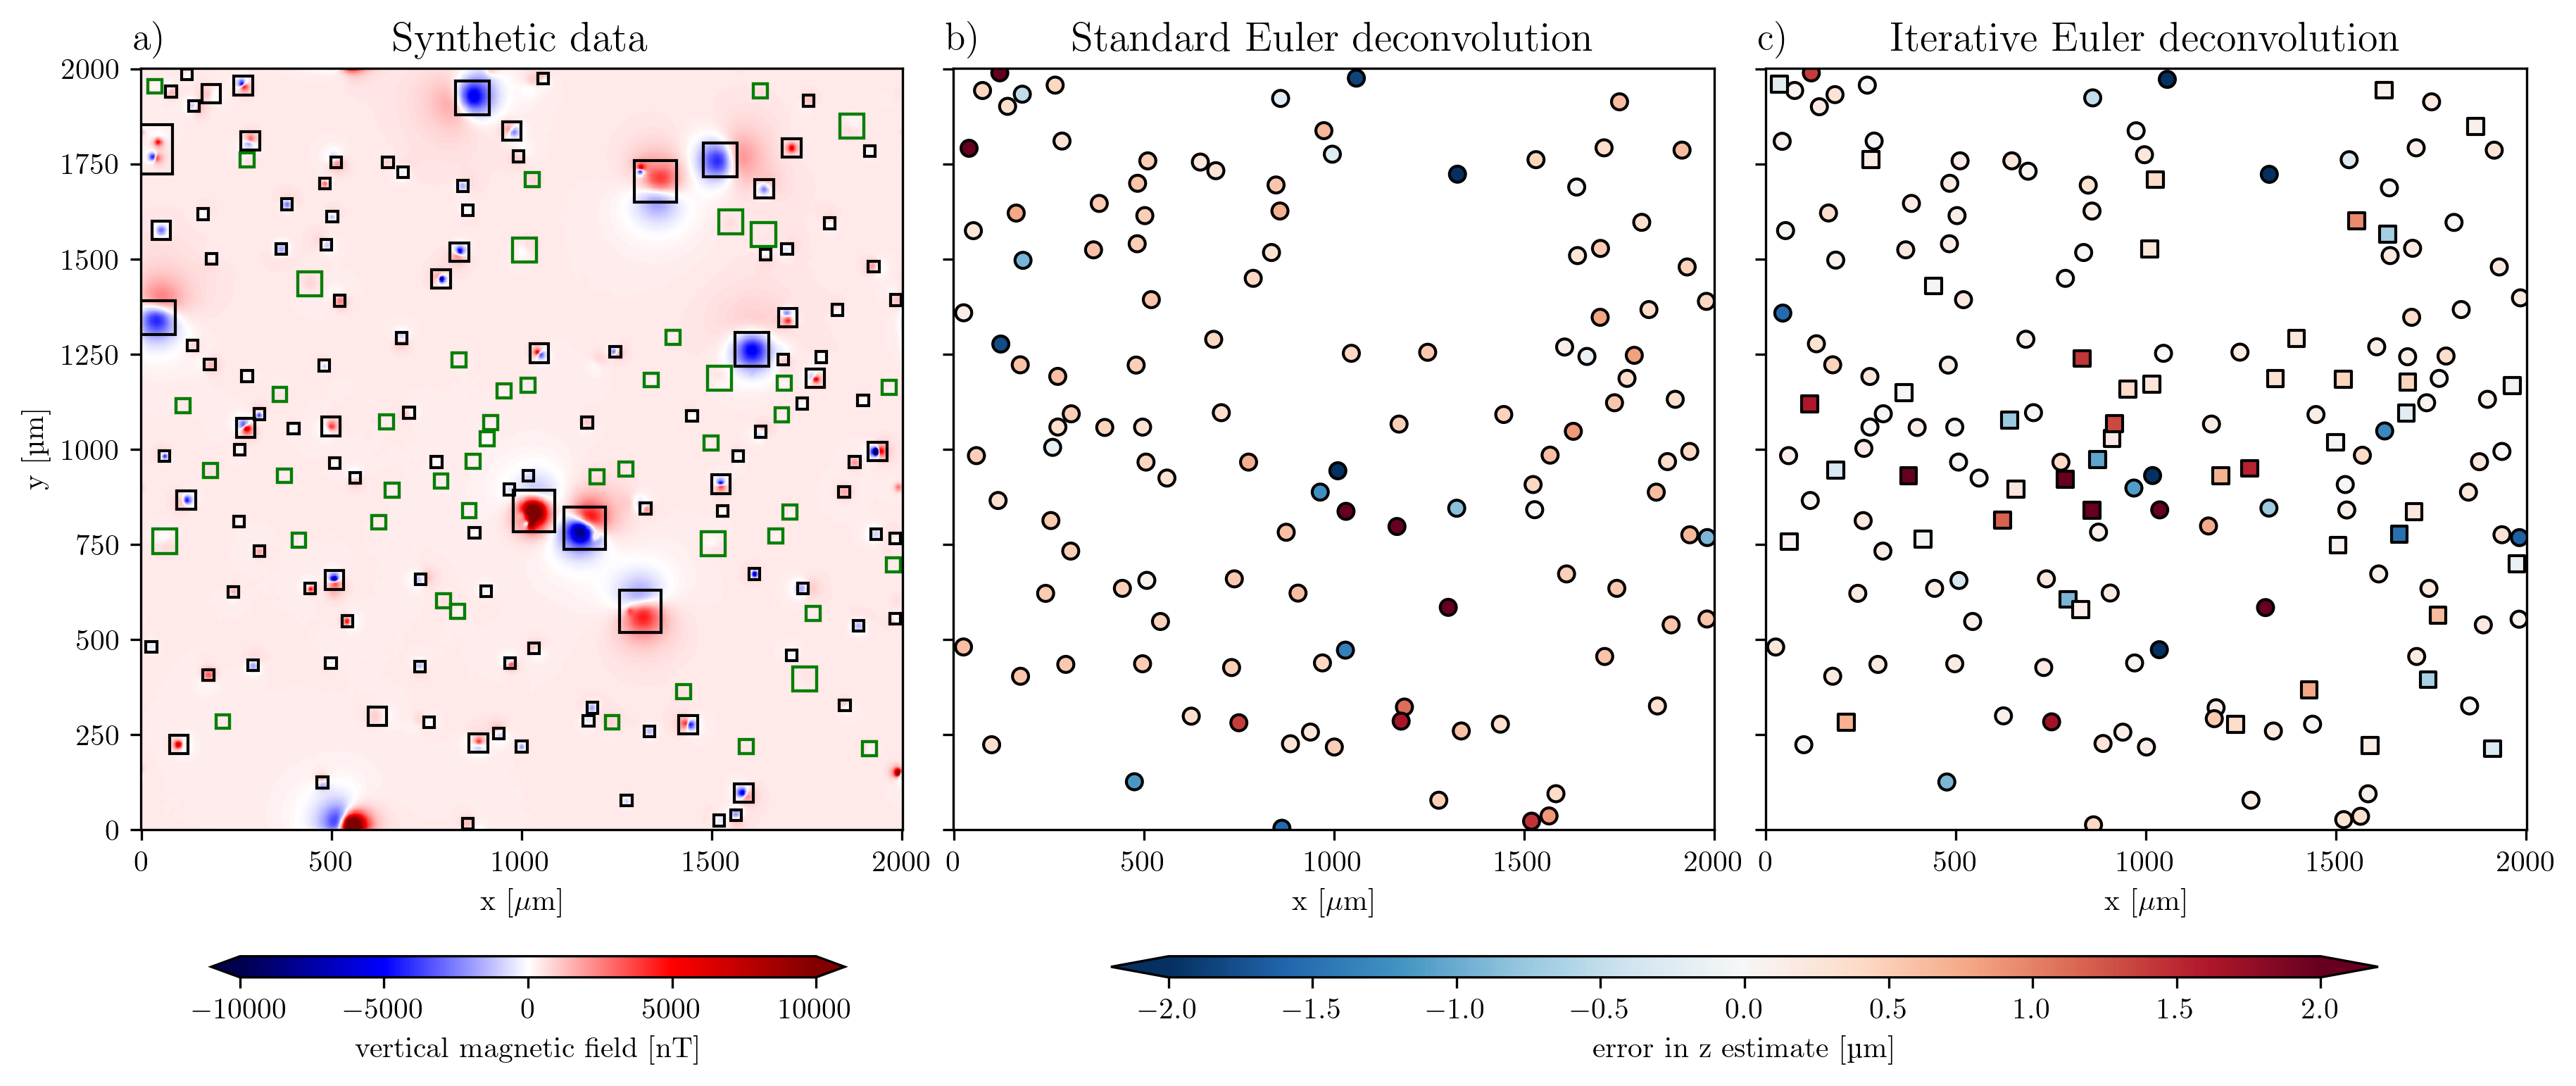
\includegraphics[width=1\linewidth]{paper/figures/euler-comparion-synthetic.png}
  \caption{Complex synthetic sample position estimation. (a) Detection window data of each magnetic source (black squares). These data windows were used in the 3D position estimation of the magnetic sources (colored circles) for the standard (b) and iterative (c) methodologies. }
  \label{euler2}
\end{figure}

These iterative Euler estimated positions were used for the magnetic inversion due to their better results except for the standard method results, which were kept unchanged from the results presented by \citet{Souza-Junior2023b}. Figure~\ref{inversion2} summarizes the comparison concerning the angular misfit, the magnetic moment misfit, and the r-squared score, respectively, for the standard (Figures~\ref{inversion2}a-c), and iterative interfering sources (Figures~\ref{inversion2}d-f). Overall, as predicted, the interfering source method outperformed the standard one in all three of the measured parameters. Nevertheless, the proposed method is fully capable of dealing with tightly clustered sources, especially for the magnetic moment misfit. This observation might have its cause inherited rooted in the limitations of the Euler deconvolution, even after all the improvement of the iterative Euler deconvolution (Figures~\ref{euler2}c), which triggers the ambiguity between the source's depth with its magnetic intensity. This example shows that the proposed methodology can be applied to magnetic microscopy yielding better results than the original method.


\begin{figure}[tb!]
  \centering
  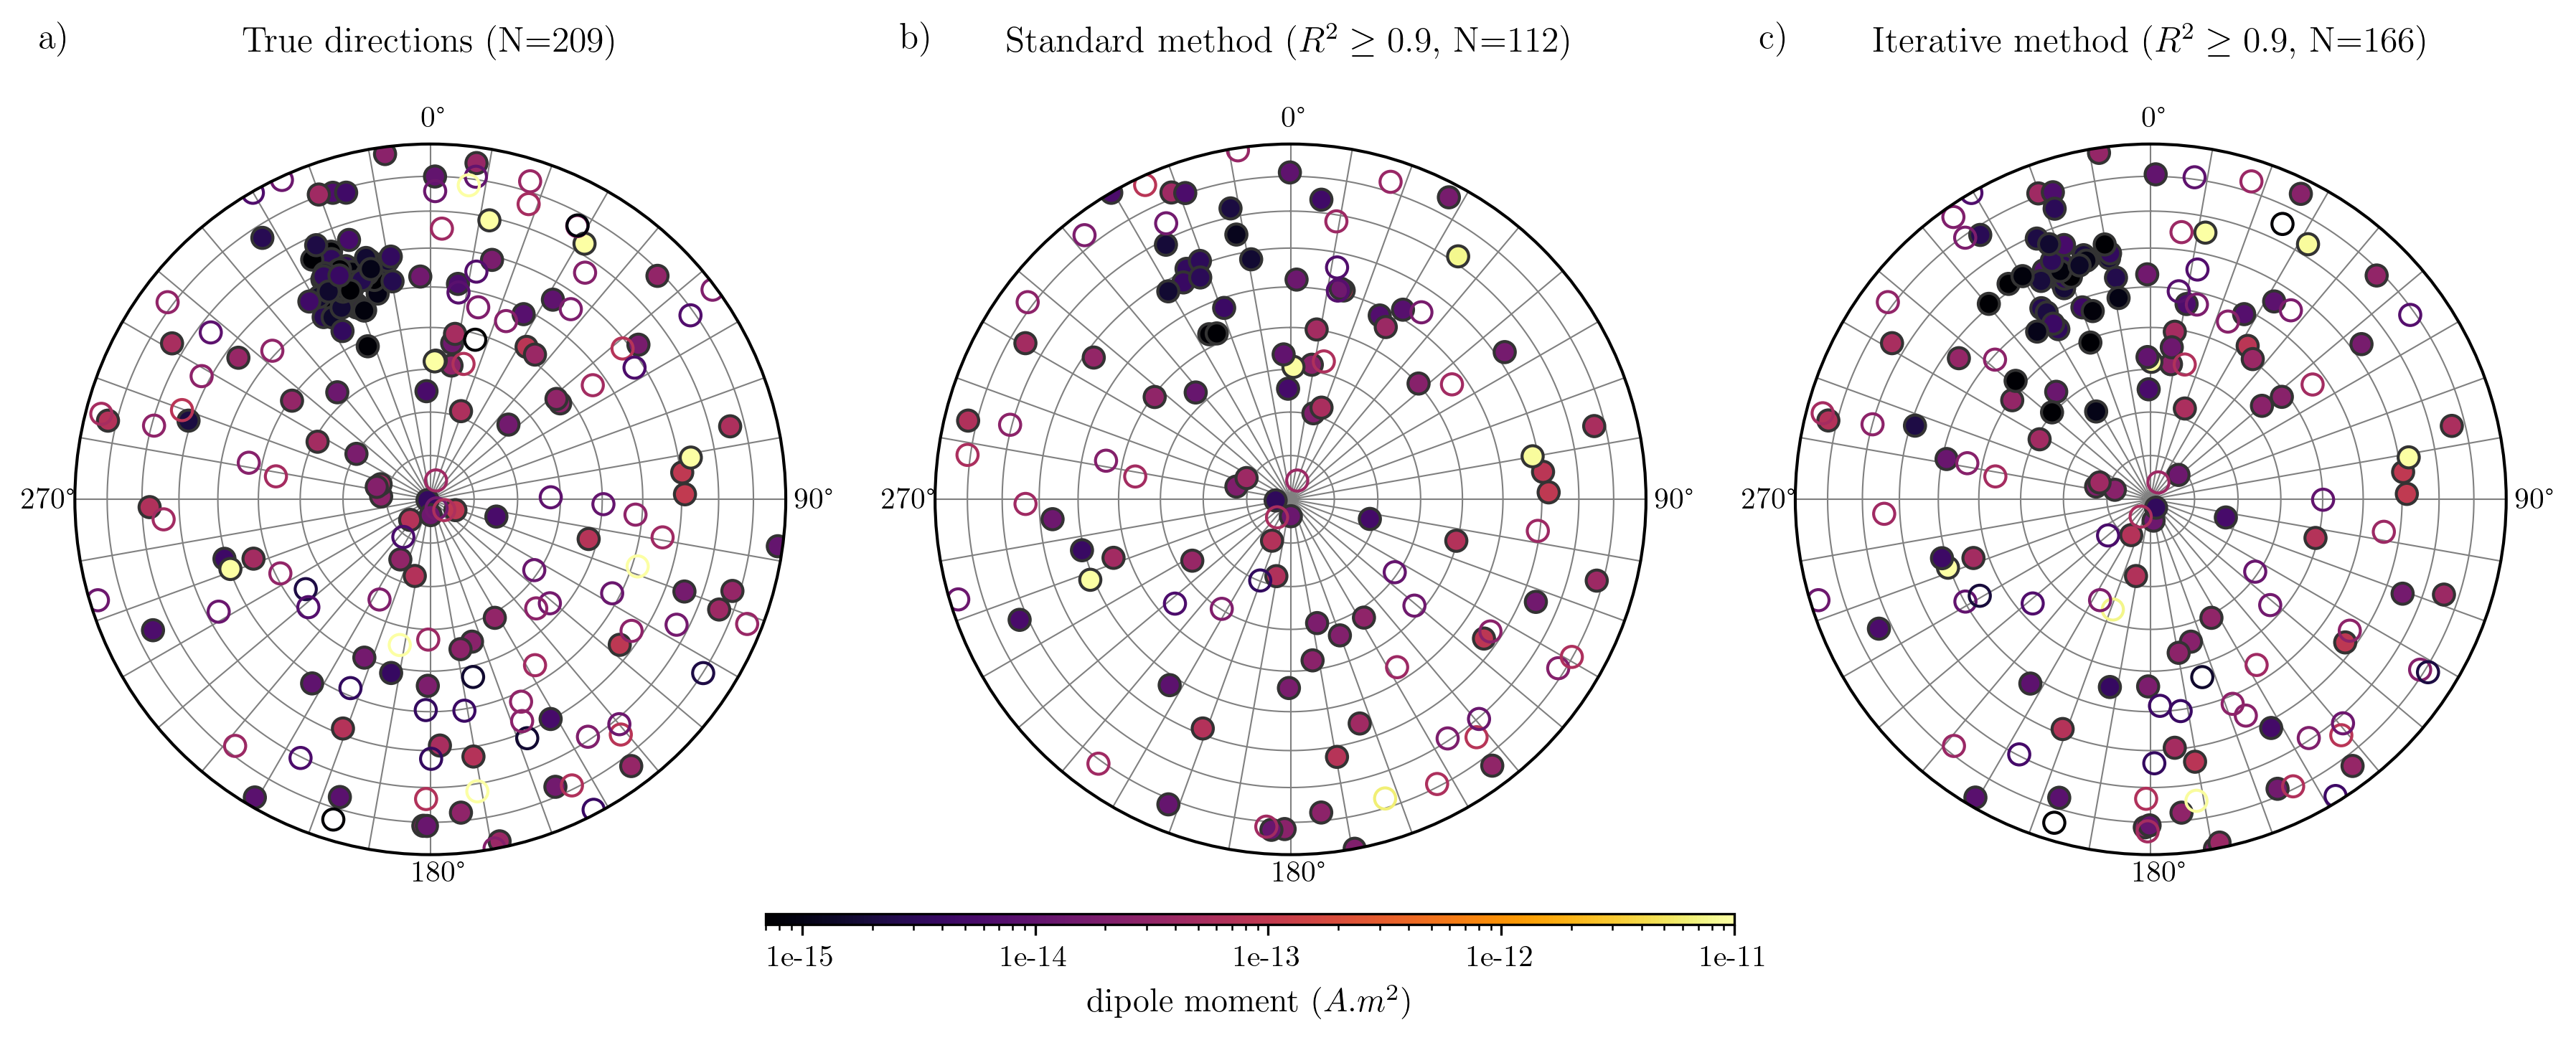
\includegraphics[width=1\linewidth]{paper/figures/synthetic-data-stereograms-comparison.png}
  \caption{Validation of the inversion results/parameters, for each particle, was obtained by computing the real and recovered differences using magnetic direction misfit, misfit of magnetic moment intensity, and the R² score from the model fitting. These parameter were calculated for the standard (a, b, and c, respectively) and iterative (d, e, and f, respectively) methodologies.}
  \label{inversion2}
\end{figure}

%%%%%%%%%%%%%%%%%%%%%%%%%%%%%%%%%%%%%%%%%%%%%%%%%%%%%%%%%%%%%%%%%%%%%%%%%%%%%%%
\section{Real data application}

To assess whether the results obtained from this new method would, in any way, yield improvements compared to what was previously demonstrated in the study by \citet{Souza-Junior2023b}, regarding the determination of magnetization directions and magnetic moment of particles in natural samples. For such, we kept the same stalagmite sample from the Wintimdouine cave in the  \citep[Agadir (Morocco),][]{Ait2019Hydro} showed in their previous study. This carbonatic rock carries both magnetite and hematite in the magnetic fabric, which was attested by thermomagnetic curves and bimodal curves of isothermal remanent magnetization (IRM) acquisition \citep{carmo2019speleothem}.

A two-step application of IRM pulse fields was employed to generate distinct orientations for both types of magnetic minerals within this sample. The initial pulse was directed in the +Y orientation with a magnitude of 2.7 T, addressing high and low-coercivity minerals. The subsequent pulse, at an intensity of 0.3 T, was directed in the -Y orientation, selectively influencing the low-coercivity minerals. This procedure ensured the development of a complex magnetization pattern, akin to the synthetic data, where hematite aligned along the +Y direction and magnetite along the -Y direction.

After remanence acquisition, the magnetic microscopy scanning technique was performed using the Quantum
Diamond Microscope (QDM) at Harvard University in a room shielded against the influence of the Earth's magnetic field. The scanned section of the sample comprised the dimensions of $\qty{1410}{\um} \times \qty{2256}{\um}$ with grid spacing of \qty{2.35}{\um} ($N = 576 \times 10^{3}$) \citep{janinedata}. The vertical component of magnetic field ($b_z$) was acquired at a constant sensor-sample distance of \qty{5}{\um}, in a background field of $< \qty{1}{\micro\tesla}$, using a spectral approach \citep{Lima2009, Fu2020, Glenn2017} as shown in Figure~\ref{real-data-euler}a. A total of 75 magnetic sources were detected by the algorithm and their positions were estimated using both the standard (Figure~\ref{real-data-euler}b) and iterative (Figure~\ref{real-data-euler}c) methodologies. At first glance, there seems to be no significant difference between the results however, but, in some cases, there are clear adjustments in the position (\textit{e.g.} towards the center of the windows).

\begin{figure}[tb!]
  \centering
  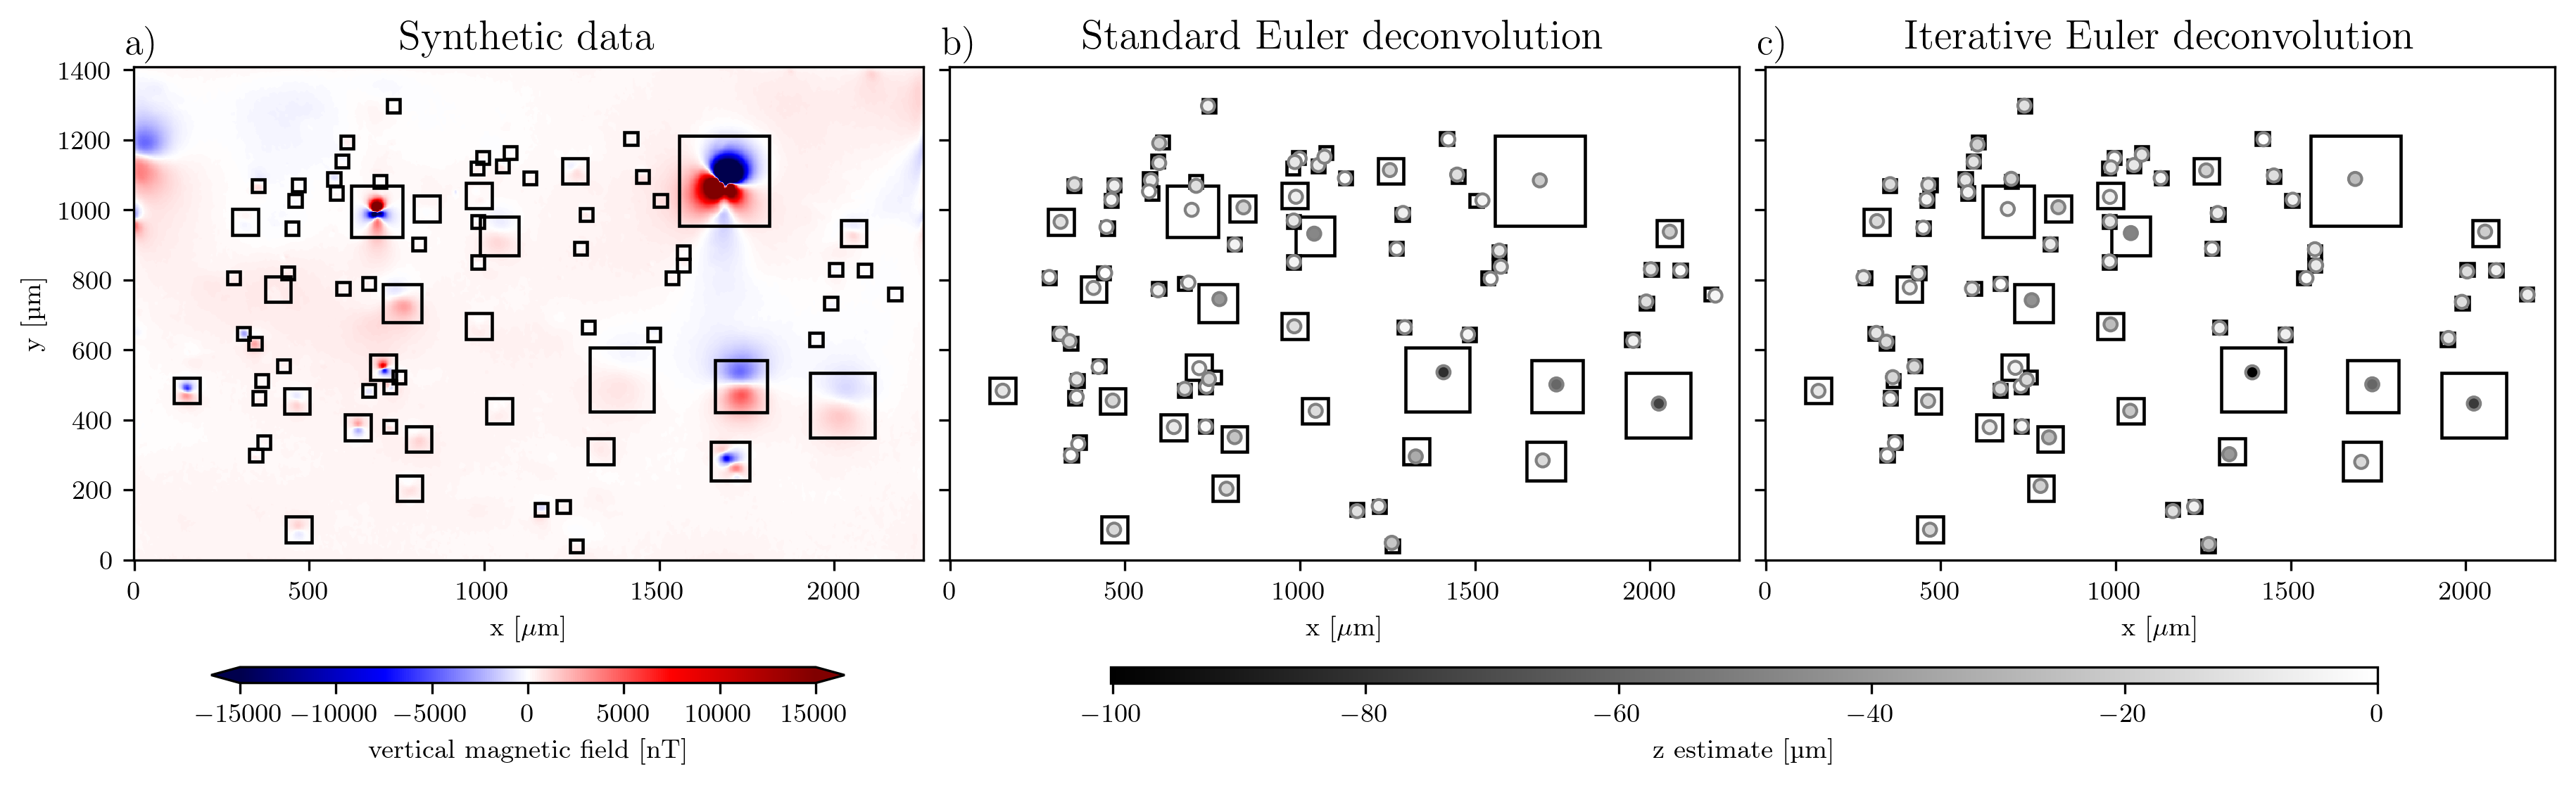
\includegraphics[width=1\linewidth]{paper/figures/euler-comparion-real.png}
  \caption{Real data sample position estimation. (a) Detection window data of each magnetic source (black squares). These data windows were used in the 3D position estimation of the magnetic sources (colored circles) for the standard (b) and iterative (c) methodologies. }
  \label{real-data-euler}
\end{figure}

Afterward, the magnetic moments and directions of all identified magnetic carriers were obtained using both methodologies. The results for the standard method do not differ from the ones presented by \citet{Souza-Junior2023b}, and the criteria for selecting the best data in the filtering process was the R-squared value \citep[similar to the dipolarity parameter,][]{Fu2020} equals to 0.85, which means that at least 85\% of the recovered data must be explained by a dipolar source. Both induced directions trends are recovered (Figure~\ref{real-data-stereograms}a), although applying the filtering criteria these directions are significantly better (Figure~\ref{real-data-stereograms}b) due to the removal of the spurious results, more often than not perfect dipolar data are also removed during the filtering process and only 46 particles pass the criteria. As mentioned earlier, one of the possible causes for this effect is the interference of stronger sources and/or shifted field, hence the reason to try the interference sources technique. The presented methodology not only yields more clustered directions within the induced field (Figure~\ref{real-data-stereograms}c) but also guarantees that the filtering criteria avoid penalizing weaker magnetic sources (Figure~\ref{real-data-stereograms}d) when compared with the original methodology. In this case, 66 magnetic sources pass the filtering criteria, thus smaller or weaker sources, but still dipolar ones, are no longer associated with low R² values. This is a clear sign of the mitigation of interference from stronger dipoles or any acquisition shifts in the magnetic field.  


\begin{figure}[tb!]
  \centering
  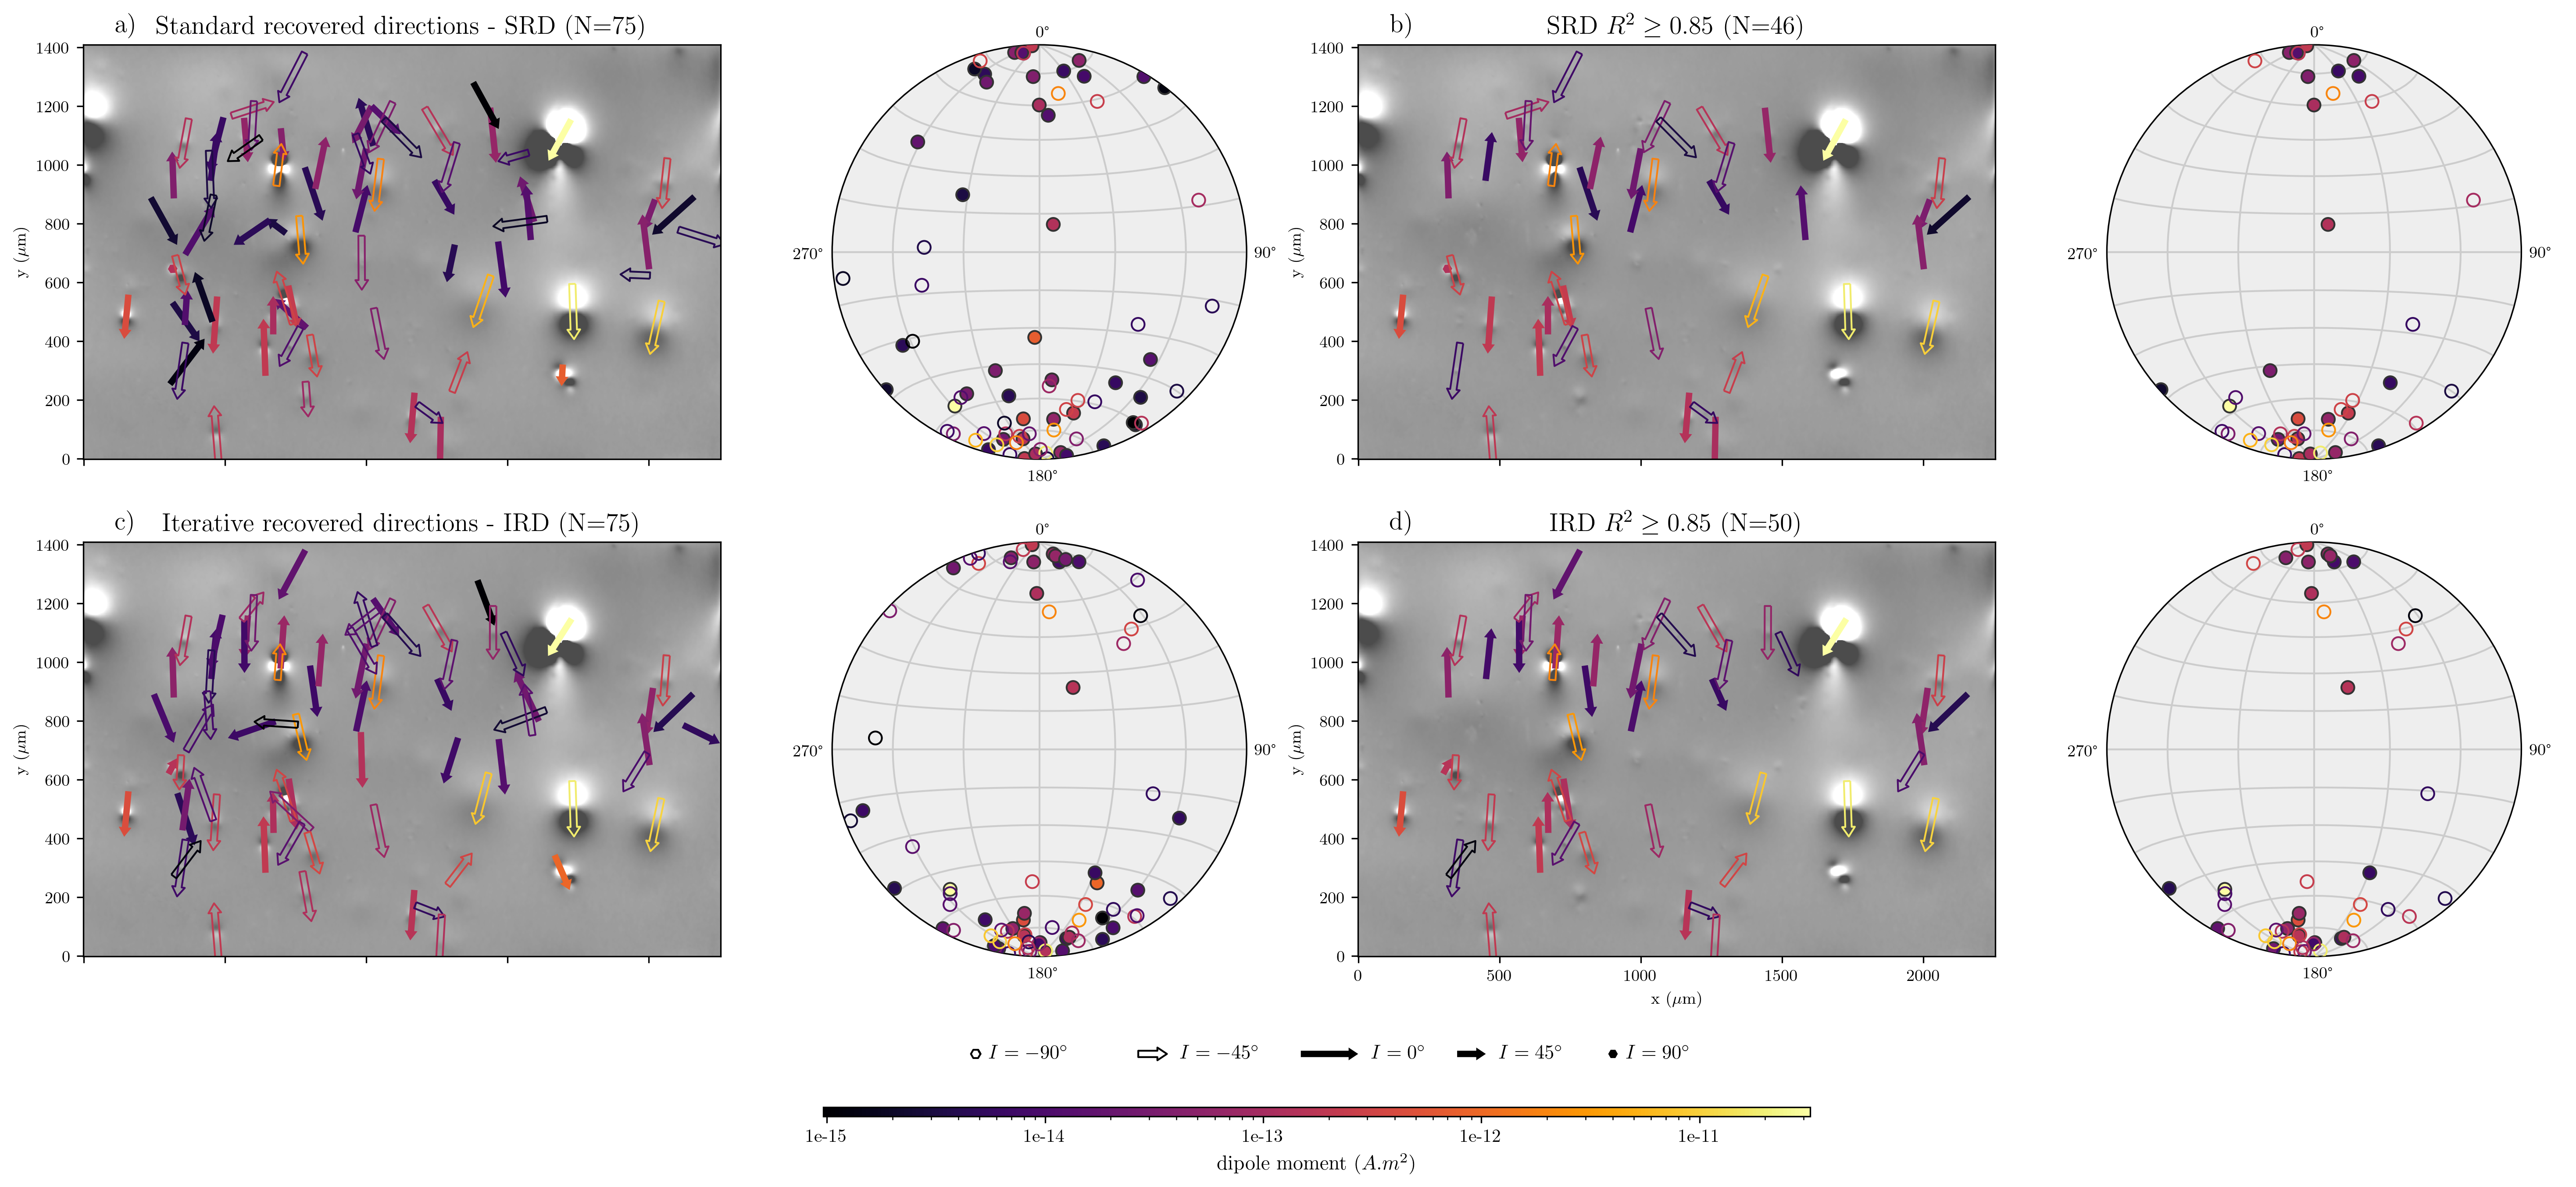
\includegraphics[width=1\linewidth]{paper/figures/real-data-stereograms.png}
  \caption{
Comparative analysis of the real data sample's estimated dipole magnetic moments and directions. Using the standard methodology: (a) all estimated directions without filtering ($N = 75$), and (b) after applying the filtering based on the coefficient of determination ($R^2 \geq 0.85$, $N = 46$). Subsequently, the iterative method was applied: (c) all estimated directions without filtering ($N = 75$), and (d) post-filtering ($R^2 \geq 0.85$, $N = 66$).
}
  \label{real-data-stereograms}
\end{figure}
%%%%%%%%%%%%%%%%%%%%%%%%%%%%%%%%%%%%%%%%%%%%%%%%%%%%%%%%%%%%%%%%%%%%%%%%%%%%%%%
\section{Discussions}

% - re-iterar que o metodo é extremamente eficiente e utiliza apenas o dado magnetic para encontrar as direcoes

% - reforçar queue é semi-automatico

% - Olhando o sintético:
%     - Falar que o código iterativo ajusta as posições das particulas (refazer a image).
%     - As direções foram drasticamente melhoradas, praticamente todas menores que 5 graus
%     - Os moments magneticos ainda dao problems por causa do erro de Euler em z
%     - Os r2 todos agoram passam no critério de filtragem
% - Olhando o real
%     - Refazer as figures posicao e adc o vetor que moveu depois do metodo iterative
%     - As direcoes de particulas mais fracas foram re-ajustadas e seguem a direções
%     - Apesar de matter os criterios de filtragem do primeiro paper, no método iterative mais partículas são retidas.





The isolated windows approach allows us to separate the area that contains the primary signal of the desired dipole, using the total gradient anomaly, and effectively excluding the region outside the window boundaries, which is less susceptible to variations in the magnetic parameters of this specific source \citep{Souza-Junior2023b}. Consequently, we omit this area from the inversion domain. With the application of this technique, it is possible to rapidly determine the 3D position and approximate the dipole moment components of numerous sources in a matter of seconds. This is similar to a method documented by \cite{Weiss2007} by applying a threshold to the long-distance interactions of individual dipoles within the magnetic microscopy data. Through this thresholding, the effect of other dipoles is negated by setting their contributions to zero. However, despite what was stated by \cite{Souza-Junior2023b}, the window segmentation seems to deviate from the core theory of the inversion problem, which mandates that the sampled area must be finite and enclosed within the inversion domain to ensure the uniqueness of results \citep{Baratchart2013, Lima2013}. This insight reveals that the windows approach is effective primarily in contexts with minimal interaction among the sources, or in situations characterized by a sparse presence of magnetic minerals, such as in the case of speleothem samples. Conversely, this approach raises significant concerns in environments with a higher density of sources, such as volcanic rocks, where interactions are more pronounced. This necessitates a thorough reexamination of the existing assumptions, highlighting the need for adaptability in the original methodology to ensure reliability during the paleomagnetic and rock magnetism studies.

Exploring the extent to which the original approach can be utilized successfully is now a critical consideration. To tackle the limitation posed by strong levels of interaction between sources, we incorporated the "interfering sources" methodology, which no longer violates the fundamental theory of the inversion problem. We aim to improve the practicality and precision of the previous approach. Our findings confirm the algorithm's efficacy in mitigating this limitation, especially in situations with prominent source interactions. In such cases, we make a trade-off between accuracy and computational time. However, it is important to note that the interfering sources methodology's efficiency remains relatively constrained when dealing with clustered sources, both for 3D position and dipole moments estimation.

The application of our methodology to synthetic data reveals promising results, particularly in the accuracy of magnetic direction determination. Nearly all our computed magnetic direction misfits are below 5 degrees (Figure~\ref{inversion2}d), indicating a significant enhancement over the original methodology. Such precision in magnetic direction estimation is a positive outcome for paleomagnetic studies. Moreover, these results satisfy a stringent filtering criterion, with R-squared values greater than or equal to 0.85 for all cases, which means that at least 85\% of the magnetic anomaly is explained by dipolar sources. This high level of model fit demonstrates the robustness of the refined methodology and suggests that it can reliably differentiate between signal and noise, providing a solid foundation for accurate magnetic moment inversion. However, a notable challenge arises when dealing with clusters of closely spaced particles. In these instances, our methodology produces erroneous amplitude results for magnetic moments (Figure~\ref{inversion2}e). We attribute this limitation to the inherited constraints from the Euler deconvolution, which also inaccurately estimates the vertical positioning of particles within clusters, even after the Euler deconvolution enhancement (Figure~\ref{euler2}c). Due to the ambiguity inherent in potential field data, the incorrect vertical positioning likely leads to the erroneous estimation of magnetic moments as the model attempts to compensate for these vertical errors. Therefore, for future paleointensity studies, it is highly recommended to use well-individualized particles to avoid these cluster-related erroneous estimations. Utilizing distinct and separate particles ensures that the magnetic signal is unambiguous, which is critical for accurate paleointensity measurements. This approach reduces the risk of overlapping signals and the potential misinterpretation that can arise from complex magnetic interactions, thus enhancing the reliability of the results obtained.

Afterward, we delve into the application of the enhanced algorithm on actual rock samples, specifically a speleothem, which was initially subjected to two opposing magnetic fields to differentiate the contributions of magnetite and hematite. This separation was observable in the original code (Figure~\ref{real-data-stereograms}a). However, the initial version did not account for some source interference effects, leading to distortions in the results. For stronger particles, this distortion was less pronounced, allowing for a satisfactory fit, as evidenced by an R-squared value greater than 0.85 (Figures~\ref{real-data-stereograms}b). Conversely, smaller or weaker particles, affected by interference from stronger sources or shifts in the measured magnetic field, showed alterations in results. These changes were reflected in the coefficient of determination and failed these particles during the filtering process. With the algorithm's improvement, the effect of these interferences was significantly diminished. Previously, 46 out of 75 particles (approximately 61.33\%) met the selection criteria. With the enhancements in the algorithm, there was a notable improvement in the particle distribution, visible by the readjustment of the smaller particles, which became less dispersed and more concentrated in the directions of the induced magnetic fields (Figures~\ref{real-data-stereograms}c). Furthermore, this improvement is reflected in the increased number of particles meeting the filtering criteria, with 66 particles (88\%) passing the threshold (Figures~\ref{real-data-stereograms}d).

This approach might represent a crucial advancement in the application of magnetic microscopy mapping for paleomagnetic studies. It addresses the critical need to identify tens of thousands of stable fine-grained particles (smaller than \SI{1}{\micro\meter}) and retrieve reliable information from magnetic images, a necessity for imparting statistical robustness to the remanence vector, as highlighted in the findings of \cite{Berndt2016}. While retaining the advantages of being a fast semi-automated approach that does not require any additional measurements. Unfortunately, our methodology also inherits the main problems pointed out by \citet{Souza-Junior2023b}, which are mainly related to the source detectability limitations. In turn, this creates opportunities for further improvements in the algorithm for source detection.

% This significant data collection effort is essential to ensure the statistical accuracy of the remanence vector, emphasizing the importance of our methodology in enhancing the precision and reliability of magnetic microscopy in paleomagnetic research.




%%%%%%%%%%%%%%%%%%%%%%%%%%%%%%%%%%%%%%%%%%%%%%%%%%%%%%%%%%%%%%%%%%%%%%%%%%%%%%%
\section{Conclusion}
% - Earth and Space Science
% - JGR Machine Learning and Computation

In conclusion, our enhanced algorithm offers significant improvements over its predecessor, particularly in magnetic microscopy mapping for paleomagnetic studies. By refining the isolation of the primary signal and integrating the "interfering sources" algorithm, we have improved the accuracy of 3D position and dipole moment estimations, addressing one of the previous code's limitations. This has led to better particle distribution and increased the number of particles meeting the filtering criteria, demonstrating more reliable magnetic signature detection. Benchmarking against the original method's outcomes substantiates the enhanced reliability and precision of our results, reinforcing the advancement of paleomagnetic data analysis and setting a definitive path for future enhancements.


%%%%%%%%%%%%%%%%%%%%%%%%%%%%%%%%%%%%%%%%%%%%%%%%%%%%%%%%%%%%%%%%%%%%%%%%%%%%%%%
\section{Open research}

% The Python source code used to produce all results and figures presented here, as well as supplemental figures and Jupyter notebooks, are available from \citet{sourcearchive}, which can also be found on \url{https://github.com/\GitHubRepository} under the MIT and CC-BY licenses.
% The QDM magnetic microscopy data are available
% from \citet{janinedata} under the CC-0 license.

% The image re-scaling and blob detection through the Laplacian of Gaussian
% methods were performed with the scikit-image library \citep{VanderWalt2014}.
% We also used matplotlib \citep{Hunter2007} and mplstereonet \citep{mplstereonet}
% for generating figures and stereograms.
% Basic calculations were performed using Numpy \citep{Harris2020} and Scipy
% \citep{2020SciPy-NMeth}.
% Verde \citep{verde2018} was used to generate data grids.
% Upward continuation was performed using Harmonica \citep{harmonica2020}.
% The Choclo library \citep{choclo2022} provided kernel functions used in the
% forward and inverse problems.
% The Numba just-in-time compilation library \citep{lam2015numba} was used to
% speed-up calculations.
% Lastly, the xarray library \citep{hoyer2017xarray} offered a fast and powerful
% tool for working with multi-dimensional datasets allowing an easy way of data
% visualization and extraction with advanced indexing techniques.



%%%%%%%%%%%%%%%%%%%%%%%%%%%%%%%%%%%%%%%%%%%%%%%%%%%%%%%%%%%%%%%%%%%%%%%%%%%%%%%
\section{Acknowledgements}

% We are indebted to the developers and maintainers of the open-source software
% without which this work would not have been possible.
% This research was supported by
% grant 162704/2021-6 from the Conselho Nacional de Desenvolvimento Científico e Tecnológico (CNPq),
% grant 2021/08379-5 from the Fundação de Amparo à Pesquisa do Estado de São Paulo (FAPESP),
% grant PRPI 22.1.09345.01.2 from Universidade de São Paulo,
% and grant IES\textbackslash{}R3\textbackslash{}213141 from the Royal Society.
% The opinions, hypotheses, and conclusions or recommendations expressed in this
% material are the responsibility of the authors and do not necessarily reflect
% the views of FAPESP.
